\documentclass[tikz,border=8pt]{standalone}
% Shared look for every TikZ diagram. Load with % Shared look for every TikZ diagram. Load with % Shared look for every TikZ diagram. Load with \input{../../tools/tikz-style.tex}
\usepackage[T1]{fontenc}
\usepackage{lmodern}
\renewcommand{\sfdefault}{lmr}  % diagrams use the same serif as the text
\usetikzlibrary{arrows.meta, positioning, shapes.geometric, calc, fit, backgrounds}
\definecolor{cblue}{HTML}{4C78A8}
\definecolor{corange}{HTML}{F58518}
\definecolor{cgreen}{HTML}{54A24B}
\definecolor{cred}{HTML}{E45756}
\definecolor{cpurple}{HTML}{B279A2}
\definecolor{cgrey}{HTML}{6B6B6B}
\tikzset{
  every picture/.style={font=\sffamily, line width=1.2pt},
  box/.style={draw=#1, fill=#1!12, rounded corners=4pt, align=center, inner sep=7pt, minimum height=1.1cm},
  box/.default=cgrey,
  arrow/.style={-{Stealth[length=3mm]}, draw=cgrey, line width=1.4pt},
  title/.style={font=\sffamily\bfseries\Large},
  note/.style={font=\sffamily\small, text=cgrey, align=center},
}
\AtBeginDocument{\hyphenpenalty=10000 \exhyphenpenalty=10000}

\usepackage[T1]{fontenc}
\usepackage{lmodern}
\renewcommand{\sfdefault}{lmr}  % diagrams use the same serif as the text
\usetikzlibrary{arrows.meta, positioning, shapes.geometric, calc, fit, backgrounds}
\definecolor{cblue}{HTML}{4C78A8}
\definecolor{corange}{HTML}{F58518}
\definecolor{cgreen}{HTML}{54A24B}
\definecolor{cred}{HTML}{E45756}
\definecolor{cpurple}{HTML}{B279A2}
\definecolor{cgrey}{HTML}{6B6B6B}
\tikzset{
  every picture/.style={font=\sffamily, line width=1.2pt},
  box/.style={draw=#1, fill=#1!12, rounded corners=4pt, align=center, inner sep=7pt, minimum height=1.1cm},
  box/.default=cgrey,
  arrow/.style={-{Stealth[length=3mm]}, draw=cgrey, line width=1.4pt},
  title/.style={font=\sffamily\bfseries\Large},
  note/.style={font=\sffamily\small, text=cgrey, align=center},
}
\AtBeginDocument{\hyphenpenalty=10000 \exhyphenpenalty=10000}

\usepackage[T1]{fontenc}
\usepackage{lmodern}
\renewcommand{\sfdefault}{lmr}  % diagrams use the same serif as the text
\usetikzlibrary{arrows.meta, positioning, shapes.geometric, calc, fit, backgrounds}
\definecolor{cblue}{HTML}{4C78A8}
\definecolor{corange}{HTML}{F58518}
\definecolor{cgreen}{HTML}{54A24B}
\definecolor{cred}{HTML}{E45756}
\definecolor{cpurple}{HTML}{B279A2}
\definecolor{cgrey}{HTML}{6B6B6B}
\tikzset{
  every picture/.style={font=\sffamily, line width=1.2pt},
  box/.style={draw=#1, fill=#1!12, rounded corners=4pt, align=center, inner sep=7pt, minimum height=1.1cm},
  box/.default=cgrey,
  arrow/.style={-{Stealth[length=3mm]}, draw=cgrey, line width=1.4pt},
  title/.style={font=\sffamily\bfseries\Large},
  note/.style={font=\sffamily\small, text=cgrey, align=center},
}
\AtBeginDocument{\hyphenpenalty=10000 \exhyphenpenalty=10000}

\begin{document}
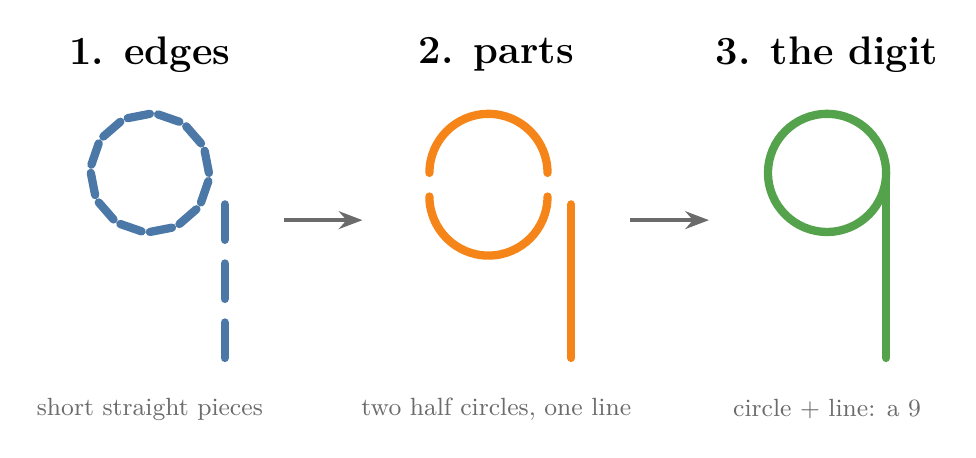
\begin{tikzpicture}[every node/.append style={font=\sffamily}]
  \tikzset{stroke/.style={line width=3pt, line cap=round, draw=#1}}
  % stage 1: edges
  \node[title] at (1.2,2.4) {1. edges};
  \foreach \a in {0,30,...,330}{ \draw[stroke=cblue] ({1.2+0.75*cos(\a)},{0.9+0.75*sin(\a)}) -- ({1.2+0.75*cos(\a+22)},{0.9+0.75*sin(\a+22)}); }
  \draw[stroke=cblue] (2.15,0.5) -- (2.15,0.05); \draw[stroke=cblue] (2.15,-0.25) -- (2.15,-0.7); \draw[stroke=cblue] (2.15,-1.0) -- (2.15,-1.45);
  \node[note] at (1.2,-2.1) {short straight pieces};
  \draw[arrow] (2.9,0.3) -- (3.9,0.3);
  % stage 2: parts
  \node[title] at (5.6,2.4) {2. parts};
  \draw[stroke=corange] (4.75,0.9) arc (180:0:0.75);
  \draw[stroke=corange] (4.75,0.6) arc (180:360:0.75);
  \draw[stroke=corange] (6.55,0.5) -- (6.55,-1.45);
  \node[note] at (5.6,-2.1) {two half circles, one line};
  \draw[arrow] (7.3,0.3) -- (8.3,0.3);
  % stage 3: whole
  \node[title] at (9.8,2.4) {3. the digit};
  \draw[stroke=cgreen] (9.8,0.9) circle (0.75);
  \draw[stroke=cgreen] (10.55,0.9) -- (10.55,-1.45);
  \node[note] at (9.8,-2.1) {circle + line: a 9};
\end{tikzpicture}
\end{document}
